\chapter{TINJAUAN PUSTAKA}
\label{chap:tinjauanpustaka}

% Ubah bagian-bagian berikut dengan isi dari tinjauan pustaka
\section{Hasil penelitian/perancangan terdahulu}
Metode Regresi Polinomial adalah sebuah metode pendekatan terhadap data-data yang telah disediakan sebelumnya. Hasil keluaran dari metode Regresi Polinomial ini berupa rumusan matematika berdasarkan data-data yang telah disediakan. Regresi polinomial dapat bekerja secara efisien meskipun dengan model yang non-linear 
\parencite{ref_regresi}. Berikut adalah rumusan dari regresi polinomial dengan satu variabel bebas: 
\begin{equation}
  y = a_0 + a_1x + a_2x^2 + \ldots + a_nx^n
\end{equation}
Dimana \(y\) adalah variabel terikat, \(x\) adalah variabel bebas, dan \(a_0, a_1, a_2, \ldots, a_n\) adalah koefisien dari regresi polinomial.

\section{Teori/Konsep Dasar}

\subsection{Kamera \emph{Omnivision}}
\label{sec:omnivision}
\begin{figure}[H]
    \centering
  
    % Ubah dengan nama file gambar dan ukuran yang akan digunakan
    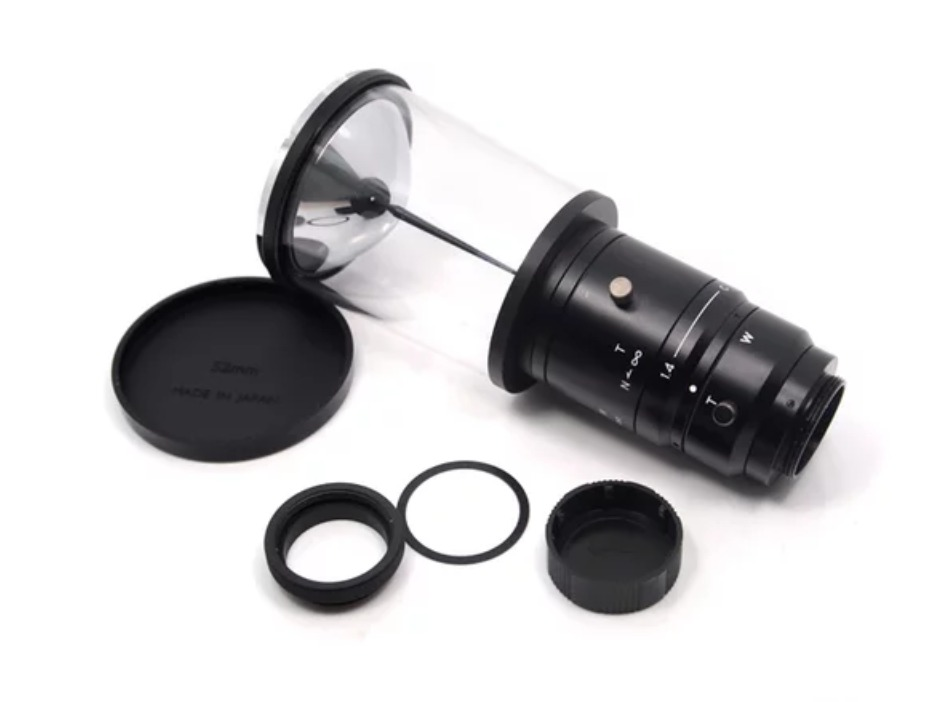
\includegraphics[scale=0.20]{gambar/omnivisino2.jpeg}
  
    % Ubah dengan keterangan gambar yang diinginkan
    \caption{Kamera Omnivsion.}
    \label{fig:omnivision}
\end{figure}
Kamera \emph{omnivision} adalah sebuah kamera yang bisa melihat 360 derajat sekitar 
kamera tersebut \parencite{ref_kamera_omni}. 
Jarak pandang kamera \emph{omnivision} tidak terbatas 
tergantung dari resolusi kamera itu sendiri dan 
konstruksi cerminnya. Pada dasarnya kamera \emph{omnivision} 
adalah kamera biasa yang ditembakkan ke sebuah cermin cembung 
sehingga pandangan kamera tersebut bisa ke segala arah. 

\subsection{Neural Network}
\label{sec:nn}
\begin{figure}[H]
    \centering
  
    % Ubah dengan nama file gambar dan ukuran yang akan digunakan
    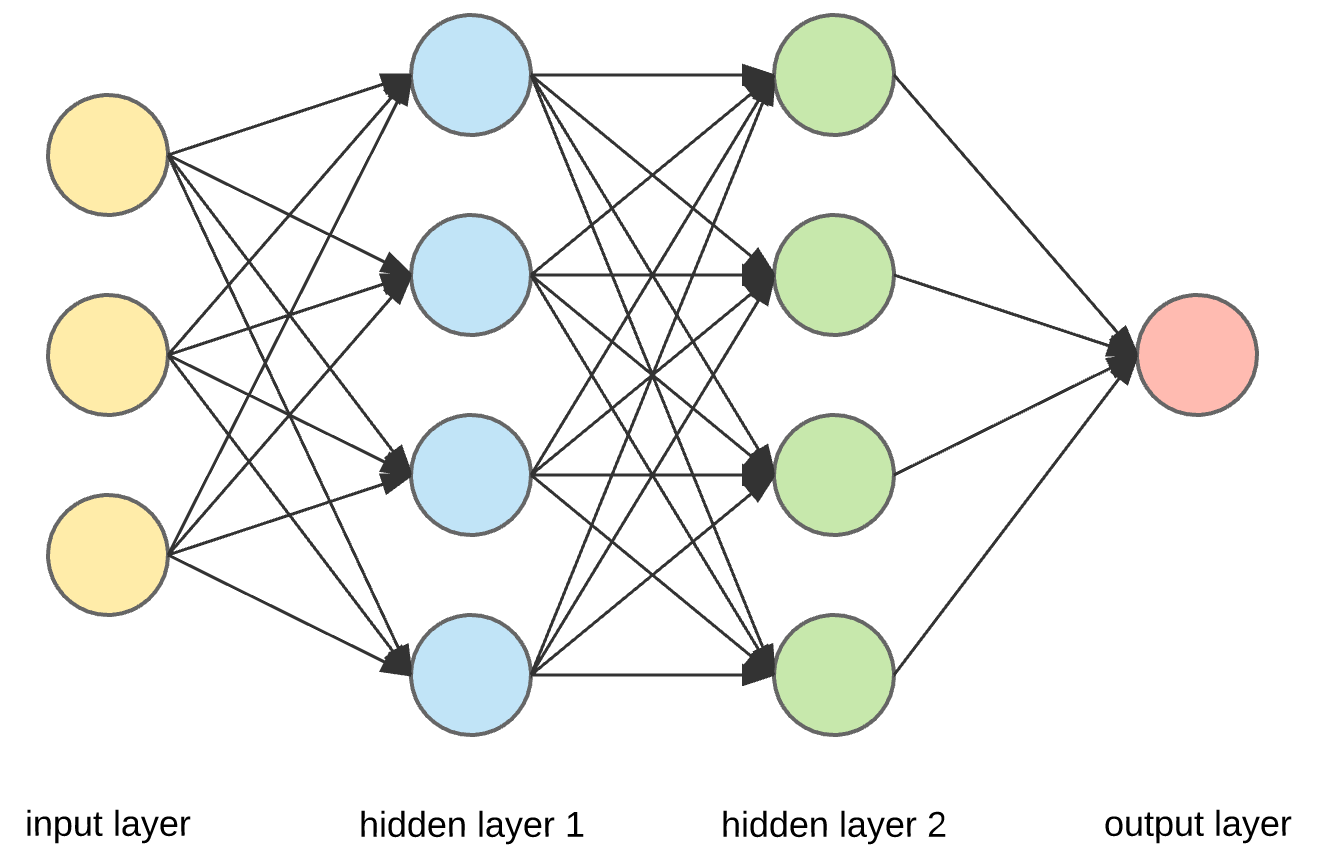
\includegraphics[scale=0.20]{gambar/nn.png}
  
    % Ubah dengan keterangan gambar yang diinginkan
    \caption{Neural Network.}
    \label{fig:nn}
\end{figure}
\emph{Neural network} merupakan bagian dari Pembelajaran Mesin. 
\emph{Neural network} diciptakan untuk mengatasi masalah ketidaklinearan 
pada sebuah model \parencite{ref_neural_network}. Pada dasarnya, 
\emph{Neural network} hanyalah sekumpulan \emph{Neuron} 
yang terhubung oleh sebuah \emph{Weight} dan \emph{Bias}. Selain 
\emph{Weight} dan \emph{Bias}, ada juga namanya \emph{forward propagation} 
menggunakan \emph{activation function} atau 
biasa disebut transfer function. Selain \emph{forward propagation},
 terdapat \emph{backward propagation} menggunakan \emph{loss function}. 

\subsection{\emph{Activation Function}}
\emph{Activation function} adalah sebuah fungsi yang digunakan untuk men-transfer 
data pada masing-masing layer pada \emph{Neural Network}. 
Dalam \emph{Neural Network}, \emph{Activation function} berperan sebagai 
\emph{forward propagation} yaitu perjalanan dari layer input menuju 
layer output. Beberapa \emph{activation Function} memiliki nilai 
saturasi biasanya bernilai 1 contohnya Sigmoid yang bernilai 
pada interval 0 sampai 1. Ada juga \emph{activation Function} lain yaitu 
tanh yang bernilai pada interval -1 sampai 1 \parencite{ref_activation_function}.

\subsection{\emph{Loss Function}}
\emph{loss function} adalah bagian dari \emph{Neural Network} 
yang bertujuan untuk memberikan umpan balik 
pada model tentang baik atau buruknya fase \emph{training}. 
\emph{loss function} pada \emph{Neural Network} bekerja pada jalur 
\emph{Backward Propagation} yaitu dari layer output menuju layer input. 
Ada beberapa macam \emph{loss function} salah satunya adalah MSE 
(\emph{Mean Squared Error}). MSE \emph{loss function} lebih baik digunakan pada 
data dengan nilai fluktuasi yang rendah \Parencite{ref_loss_function}. 

Selain \emph{loss function}, ada sebuah teori lagi yaitu Optimizer. 
Optimizer adalah sebuah algoritma yang bisa digunakan untuk menentukan 
\emph{learning rate} sistem training. \emph{Learning rate} pada 
\emph{Neural Network} digunakan untuk mengatur seberapa cepat model 
akan konvergen terhadap data-datanya. 

\subsection{\emph{Mobile Robot}}
\label{sec:mobile_robot}
\begin{figure}[H]
    \centering
  
    % Ubah dengan nama file gambar dan ukuran yang akan digunakan
    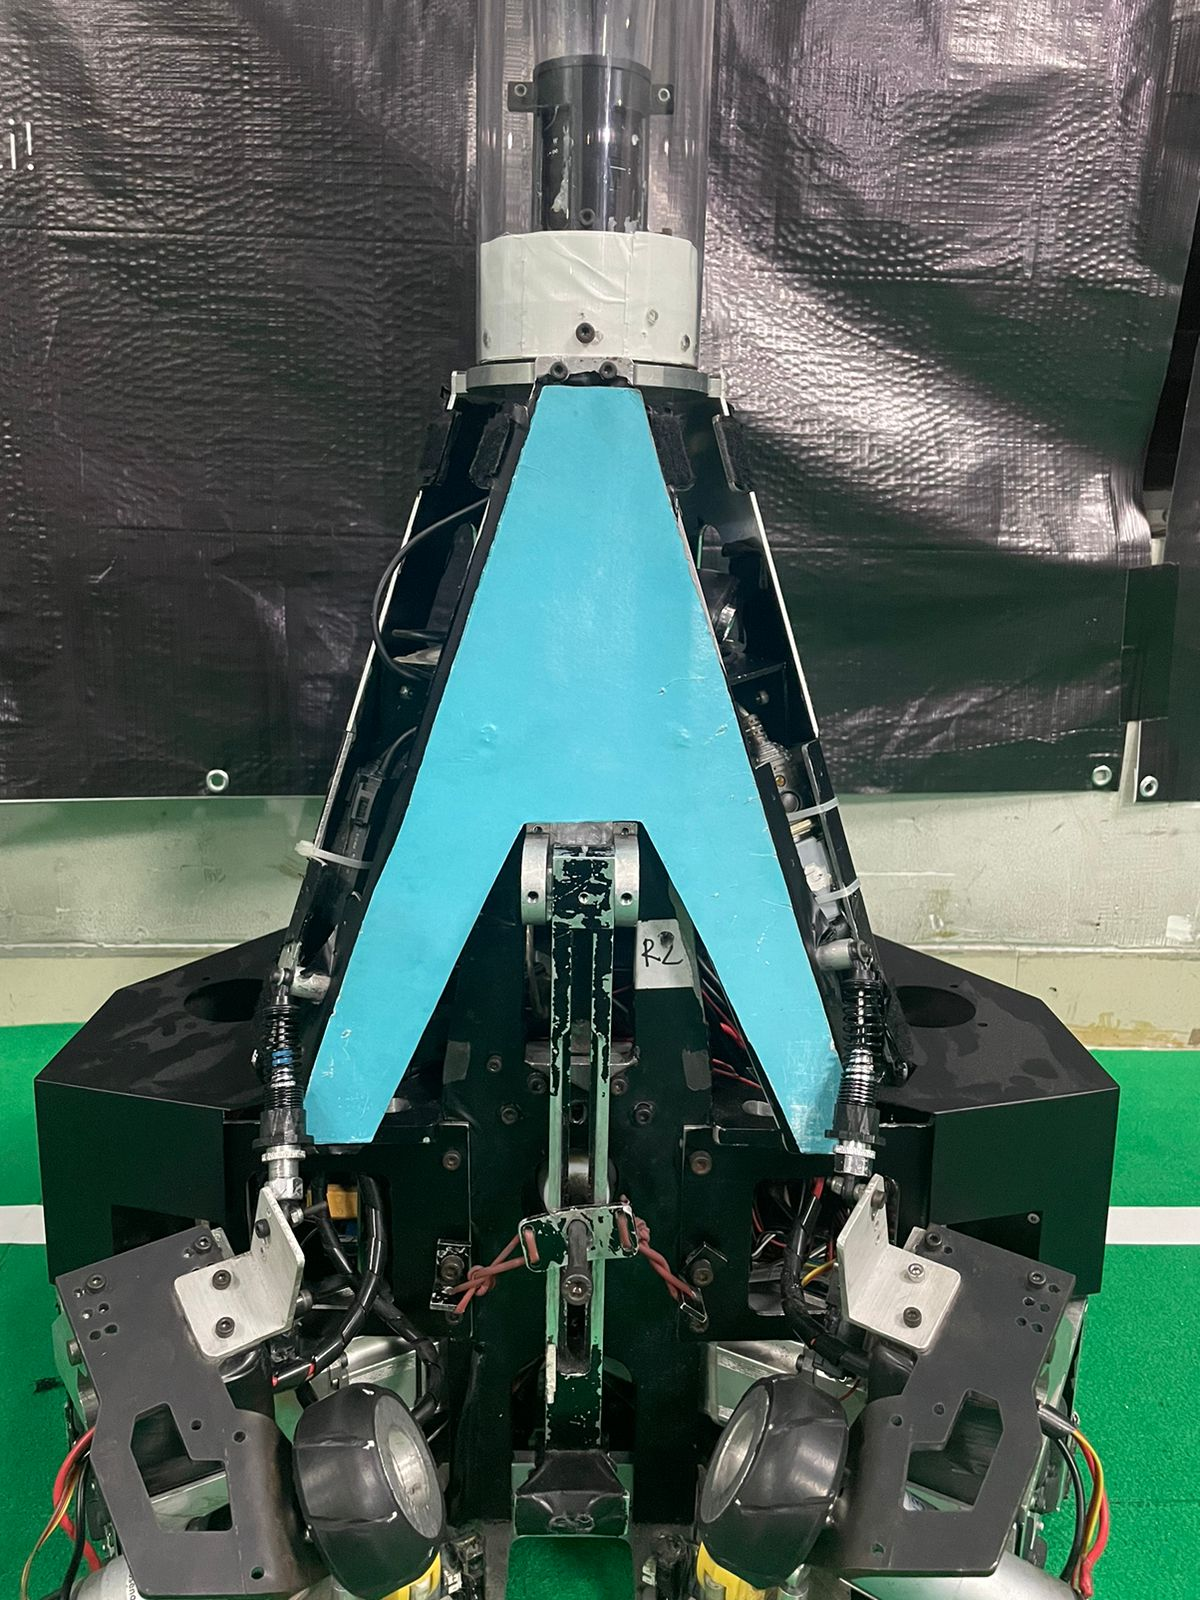
\includegraphics[scale=0.10]{gambar/iris1.jpeg}
  
    % Ubah dengan keterangan gambar yang diinginkan
    \caption{Robot IRIS tampak depan.}
    \label{fig:mobile_robot}
\end{figure}
\emph{Mobile Robot} adalah sebuah robot yang didesain agar bisa bergerak 
atau berpindah tempat dengan mudah. Performa \emph{Mobile Robot} banyak 
dikhususkan pada sistem tracking, lokalisasi, dan algoritma. Ketiga 
hal tersebut berdasar pada kemampuan sensing yang baik \Parencite{ref_mobile_robot}. 
Pada umumnya, sensor yang digunakan adalah kamera baik itu kamera biasa 
maupun kamera \emph{omnivision}. Penggunaan kamera \emph{omnivision} dapat 
membuat robot melihat ke segala arah, Namun pre-processing datanya yang 
lebih sulit dibandingkan dengan kamera biasa.

\subsection{\emph{OpenCV}}
\label{sec:opencv}
\begin{figure}[H]
    \centering
  
    % Ubah dengan nama file gambar dan ukuran yang akan digunakan
    
\includegraphics[scale=0.40]{gambar/opencv.png}
  
    % Ubah dengan keterangan gambar yang diinginkan
    \caption{Logo OpenCV.}
    \label{fig:opencv}
\end{figure}
\emph{OpenCV} adalah library open-source yang dikembangkan oleh 
Intel dengan bahasa pemrograman C/C++. 
\emph{OpenCV} menyediakan banyak algoritma yang berhubungan dengan Visi 
Komputer \Parencite{ref_opencv}. OpenCV banyak digunakan untuk deteksi 
objek baik itu berdasarkan warna, bentuk, ukuran, dan lain lain 
sesuai kebutuhan program. 

\subsection{Robot Operating System}
\label{sec:ros}
\begin{figure}[H]
    \centering
  
    % Ubah dengan nama file gambar dan ukuran yang akan digunakan
    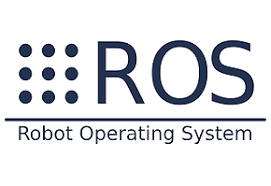
\includegraphics[scale=0.45]{gambar/ros.png}
  
    % Ubah dengan keterangan gambar yang diinginkan
    \caption{Logo ROS.}
    \label{fig:ros}
\end{figure}
ROS atau \emph{Robot Operating System} adalah sebuah platform yang berdiri 
diatas 
Linux dan berguna untuk sinkronisasi bagian bagian dari 
robot \Parencite{ref_ros}. ROS banyak digunakan sebagai inti 
pemrosesan data dari sebuah robot mulai dari pemrosesan data sensor 
hingga menjadi data aktuator. ROS menyediakan konsep modular programming 
dengan metode publish/subscribe untuk IPC (\emph{Inter Process Communication}) nya. Selain memudahkan untuk 
transfer data antar proses, ROS juga menyediakan timer dengan scheduler 
default nya mengikuti Default Linux Scheduler yaitu Priority-based scheduler. 
Hal itu memungkinkan pengguna untuk mengatur prioritas masing-masing bagian 
dari robotnya. 

\subsection{Websocket}
Websocket adalah jenis protokol komunikasi berbasis protokol TCP (\emph{Transmission Control Protocol}). 
Protokol websocket membuat kedua pengirim dan menerima untuk selalu 
membuka socket nya agar bisa saling komunikasi. 
Dibandingkan dengan HTTP (\emph{Hypertext Transfer Transfer Protocol}), 
protokol Websocket memiliki 
latensi yang lebih baik \Parencite{ref_websocket}. Aplikasi 
websocket banyak digunakan untuk aplikasi obrolan (chat), game online,
 aplikasi yang membutuhkan data \emph{realtime}, dan masih banyak lainnya. 
